% Обзорная статья по визуальным языкам программирования роботов, часть большой статьи "Применение DSM-платформы QREAL при разработке среды программирования роботов QReal:Robots", скорее всего, для сборника "Компьютерные инструменты в образовании".
% Идея: есть интересная и важная область применения визуального программирования и DSM-подхода --- программирование роботов. Существует несколько технических решений, но нет научных статей, описывающих предметную область и эти решения именно с точки зрения визуального программирования, надо восполнить недостаток. Статья --- как фундамент и problem statement для исследований в области DSM для роботов.
% Фокус: Обзор предметной области и существующих визуальных сред программирования роботов, включая QReal:Robots, сугубо с пользовательской точки зрения.
% Scope: Средства визуального программирования для роботов, их применение в школах.
% Целевая аудитория: Специалисты, занимающиеся исследованиями в области DSM, Люди, внедряющие роботов в образовательный процесс.

\documentclass[a4paper]{article}
\usepackage[a4paper, top=17mm, bottom=17mm, left=17mm, right=17mm]{geometry}
\usepackage[utf8]{inputenc}
\usepackage[T2A,T1]{fontenc}
\usepackage[colorlinks,filecolor=blue,citecolor=green,unicode,pdftex]{hyperref}
\usepackage{cmap}
\usepackage[english,russian]{babel}
\usepackage{amsmath}
\usepackage{amssymb,amsfonts,textcomp}
\usepackage{color}
\usepackage[usenames,dvipsnames,svgnames,table]{xcolor}
\usepackage{array}
\usepackage{hhline}
\hypersetup{colorlinks=true, linkcolor=blue, citecolor=blue, filecolor=blue, urlcolor=blue, pdftitle=1, pdfauthor=, pdfsubject=, pdfkeywords=}
\usepackage{graphicx}
\usepackage{indentfirst}
\usepackage{cite}
\usepackage{literat}

\sloppy
\pagestyle{plain}

\title{Реализация визуальных средств программирования роботов для изучения информатики в школах}

\author{Ю.В.Литвинов \\ ст. преп. кафедры системного программирования СПбГУ, \\ инженер-программист ЗАО <<Ланит-Терком>> \\ yurii.litvinov@gmail.com}
\date{}
\begin{document}

\maketitle
\thispagestyle{empty}

\renewcommand{\thefootnote}{}
\footnote{\small{\copyright~Ю.В.Литвинов,~2012.}}
\renewcommand{\thefootnote}{\arabic{footnote}}
\setcounter{footnote}{0}

\begin{quote}
\small\noindent
В настоящее время в школах Российской Федерации для преподавания информатики активно используется робототехнический конструктор Lego Mindstorms NXT. Этот конструктор позволяет собирать и программировать роботы, использующие моторы и сенсоры для взаимодействия с внешним миром. Однако для эффективного использования роботоконструкторов на уроках информатики требуются средства программирования создаваемых с его помощью роботов, причём эти средства должны быть доступны школьникам, никогда не программировавшим ранее. В данной статье формулируются требования к средствам визуального программирования роботов, предназначенных для применения в школах, делается обзор таких средств, интегрированных с  Lego Mindstorms NXT, и описывается новое подобное средство --- QReal:Robots.
\end{quote}

\section*{Введение}
В школьной информатике активно используется понятие <<исполнитель>> --- некая сущность, которая выполняет написанные в программе команды. Для разработки таких <<исполнителей>> традиционно используются робототехнические конструкторы, самым популярным из которых на данный момент является конструктор Lego Mindstorms NXT~\cite{legoNxt}. Он позволяет из блока управления, моторов, сенсоров и соединительных деталей собирать роботов, способных под управлением программы взаимодействовать с окружающим миром.

Существует довольно много систем, позволяющих программировать таких роботов --- как текстовые, так и визуальные. В текстовых средах, как правило, применяются языки программирования, похожие на язык C, поэтому они слишком сложны для первоначального обучения информатике в младших и средних классах школы. С педагогической точки зрения более интересны визуальные средства программирования роботов, пользоваться которыми могут даже дошкольники, не умеющие ещё читать. В данный момент для программирования роботов используются следующие средства визуального программирования: Robolab~\cite{robolab}, NXT-G~\cite{nxtG}, Microsoft Robotics Developer Studio~\cite{mrds} и QReal:Robots~\cite{robots} . 

В данной  статье проводится анализ перечисленных сред с точки зрения их пригодности для преподавания информатики и кибернетики в школах, делаются выводы об их достоинствах и недостатках, приводится описание созданной под руководством автора этой работы среды QReal:Robots, определяются направления дальнейшего развития подобных систем.

\section{Использование визуального программирования роботов в школах}
Идея использовать роботов при начальном обучении информатике родилась неслучайно. Проблема, на которую указывал ещё Ф.~Брукс в своей известной статье <<Серебряной пули нет>>~\cite{mythicalManMonth}, заключается в том, что программы нематериальны, их невозможно увидеть. Кроме того, даже представить себе программу не так просто --- каждый человек <<видит>> программу по-разному. Людям, которые программируют впервые, приходится сразу же работать с абстрактными понятиями, и судить о правильности своих программ они могут только по внешним проявлениям их работы --- какой ответ программа выведет на экран. При этом может быть совсем не очевидно, как программа работает, и что делать, если выводимый ею ответ неправильный, что нужно делать, чтобы получить правильный ответ. К тому же часто случается так, что программа работает неправильно, но правильный ответ всё-таки выводит. Всё это делает изучение информатики весьма сложным.

И отечественные, и зарубежные методисты давно осознают эту проблему, поэтому традиционно начальное обучение информатике проводится с использованием концепции <<исполнителя>> --- некоторого, зачастую воображаемого, устройства, способного выполнять простые команды в некотором простом окружении. Один из самых известных исполнителей, применяемых в школах --- <<черепашка>> LOGO~\cite{logo}, разработанная американским программистом, психологом и педагогом Сеймуром Пейпертом в 1967 году. Исполнитель <<черепашка>> может перемещаться по экрану, оставляя за собой след, которым вычерчиваются различные фигуры. Черепашка подчиняется командам простого интерпретируемого языка, позволяющего описывать её перемещения и повороты. Таким образом, процесс исполнения программы визуализируется движением исполнителя по экрану, и если программа работает неправильно, это будет сразу видно. 

В Советском Союзе преподавание информатики как школьного предмета началось во многом благодаря усилиям академика А.П.~Ершова и его коллектива, в который входили Г.А.~Звенигородский и Н.А.~Юнерман. Ими была разработана отечественная учебная система <<Робик>>~\cite{robik}, основанная в основном на тех же принципах, что и Logo. Ими же были разработаны методики и программы преподавания информатики в школах, где понятие <<исполнитель>> занимало ключевую позицию.

Однако исполнитель, перемещающийся по экрану, всё же недостаточно нагляден. Сеймур Пейперт в своих экспериментах использовал механическую черепашку~\cite{logoTurtle} --- реальный, материальный объект, исполняющий программу, что оказалось гораздо понятнее для школьников, чем черепашка, движущаяся по экрану. Современные технологии позволяют создавать недорогие механические устройства, управляемые загружаемой в них программой либо непосредственно с компьютера, поэтому идея использования материальных исполнителей в школьной информатике получила второе рождение, из-за чего получил распространение конструктор Lego Mindstorms NXT (методические рекомендации по использованию этого конструкора в школах можно найти, например, в пособии~\cite{filippov}). 

Робототехнический конструктор довольно сложно программировать. Из набора деталей могут быть собраны самые разные конструкции, поэтому программировать приходится в терминах оборотов моторов, подключённых к определённым портам управляющего блока, а не в терминах движений и поворотов. Это, безусловно, делает процесс обучения более творческим, поскольку школьники могут собрать своего собственного исполнителя, но и более сложным с точки зрения написания для этого исполнителя программ. Проблема сложности программирования преодолевается использованием наглядных визуальных языков и удобных графических редакторов для составления программ из блоков, представляющих элементарные команды, такие как <<включить мотор>>, <<гудок>> и т.д. Таким образом, начинающие работают с графическими языками программирования, а более опытные школьники постепенно переходят на текстовые C-образные языки. В комплекте с конструктором поставляется графическая среда программирования NXT-G, поэтому визуальные языки среди использующих Mindstorms NXT весьма популярны.

\section{Требования к средствам программирования роботов}
Определим требования, которым, на наш взгляд, должны удовлетворять средства программирования роботов для того, чтобы они были успешно применимы в школах в преподавании информатики.
\begin{itemize}
  \item Возможность создавать довольно сложные программы, включающие в себя нетривиальные математические выражения, циклы, ветвления, переменные, параллельные задачи --- применение таких средств должно дать возможность иллюстрировать содержательный материал из информатики и кибернетики, например, понятие регуляторов.
  \item Простота и удобство в работе. Неудобный пользовательский интерфейс создаёт дополнительную когнитивную нагрузку на школьников и усложняет восприятие и без того сложного материала.
  \item Наличие встроенных средств отладки для того, чтобы школьники могли следить за ходом выполнения своей программы и её состояниями и имели бы инструмент для эффективного поиска ошибок.
  \item Возможность перехода от графической формы программы к текстовой, чтобы школьники старших классов, серьёзно занимающиеся программированием, имели возможность смотреть на то, как их программа выглядит на более приближенном к индустриальному программированию текстовом языке, а также имели бы возможность вносить в программу правки в той же среде, в которой они привыкли работать.
  \item Необходима русскоязычная среда разработки, поскольку школьники зачастую ещё не владеют иностранными языками, а необходимость работать со словарём существенно усложняет восприятие материала.
  \item Цена --- каким бы хорошим ни был продукт, если он стоит дорого, не все российские школы могут себе его позволить.
  \item Поддержка и развитие --- желательно, чтобы продукт продолжал развиваться и адаптироваться к новым операционным системам и аппаратному обеспечению.
\end{itemize}

\section{Среда NXT-G}
Среда NXT-G~\cite{nxtG} --- единственное средство программирования, которое поставляется в комплекте с конструктором Lego Mindstorms NXT. Эта среда основана  на системе визуального программирования LabView~\footnote{LabView home page, www.ni.com/labview/} от компании National Instruments. В LabView в качестве языка программирования используется визуальный язык G. Язык G моделирует процесс вычислений, ориентированный на данные, в котором явно задаются связи между блоками по данным, а не последовательность выполнения операторов. Блок программы может также выдавать выходные данные, которые могут служить входными для другого блока. Блоки начинают исполняться, когда имеют данные на всех своих входах. Если сразу несколько блоков имеют данные на всех входах, то они исполняются параллельно. Такой подход довольно сильно отличается от принятого в императивном программировании, но тем не менее он широко распространён среди инженеров и учёных. Например, на тех же принципах основана другая известная визуальная среда программирования научных вычислений и моделирования --- Matlab/Simulink~\footnote{Simulink product page on the MathWorks website, http://www.mathworks.com/products/simulink/?s\_cid=wiki\_simulink\_8}.

Основная проблема этой среды заключается в довольно слабой поддержке математических выражений. Математические формулы здесь, как и вся программа, строятся из блоков: есть блоки арифметических операций, блоки чтения и записи значения в переменную, блок, считывающий значение константы, блоки, считывающие показания с сенсоров и т.д. Таким образом для того, чтобы запрограммировать даже несложную формулу, требуется изображать блоками дерево разбора выражения, которое эту формулу задаёт. Таким образом, первому из предложенных требований --- пригодности для иллюстрации содержательного материала информатики и кибернетики --- NXT-G не соответствует. В основном поэтому NXT-G и не получил широкого распространения в школах.

Что касается простоты и удобства в работе, то среда NXT-G специально создавалась для начинающих и поэтому довольно эргономична. По мнению некоторых пользователей она даже слишком эргономична, поскольку не даёт произвольно размещать блоки на диаграмме, автоматически (и не всегда удачно) прокладывает соединительные линии между блоками и т.д. Для применения NXT-G в школьных классах оказалась важна ещё такая его особенность: большая часть свойств элементов не отображается на диаграмме, а доступна только через редактор свойств, что делает невозможным показ всей программы на проекторе. Никаких средств отладки NXT-G не имеет, текстовая форма программы не порождается, русификация существует, но не входит в официальную поставку системы. К достоинствам  продукта следует отнести то, что он распространяется вместе с конструктором и доступен для скачивания с сайта производителя бесплатно. Кроме того, продукт до сих пор развивается и обновляется. Средствами LabView возможно добавление сторонних блоков, кроме того, сам NXT-G позволяет выделить набор блоков в подпрограмму и использовать её как новый блок.

\section{Среда Robolab}
Среда Robolab~\cite{robolab} так же как и NXT-G основывается на продукте LabView. Эта среда специально создавалась для школьного образования и c самого начала ориентировалась на потребности школьных учителей и специфику преподавания в школах. В частности, возможности Robolab разбиты на несколько уровней. На самом простом уровне доступны только некоторые возможности, программа строится путём заполнением пустых мест в шаблоне, а также посредством выбора блоков из всплывающего меню. Это позволяет создавать только самые простые программы, имеющие стандартную структуру: команды управления моторами, за которыми следует блок, ожидающий наступления какого-либо события. Причём этот уровень имеет четыре подуровня, и на первых трёх подуровнях программа может состоять только из одного такого <<шага>>. Сделано всё это для того, чтобы дать возможность детям в начальной школе или даже детском саду пользоваться этой программой --- в столь раннем возрасте они вполне могут не уметь читать. На втором уровне (который тоже состоит из нескольких подуровней) пользователи могут рисовать уже настоящие диаграммы, размещая произвольным образом блоки из палитры и соединяя их линиями, определяющими поток управления. Разница между подуровнями заключается в количестве доступных в палитре блоков, первые подуровни имеют меньше блоков с меньшим количеством параметров. Разбиение на уровни и подуровни организовано так, чтобы дети могли осваивать среду программирования практически без помощи учителя, руководствуясь лишь интуицией. Отзывы учителей, приведённые в~\cite{robolab}, показывают, что этой цели удалось достигнуть.

Математические выражения Robolab поддерживает гораздо лучше, чем NXT-G --- их можно задавать в обычном текстовом виде, имеется возможность использовать тригонометрические функции, обращаться напрямую к значениям показаний сенсоров и т.д. Циклы в Robolab реализованы довольно необычно: есть блок <<метка>> и блок <<переход к метке>>, передача управления больше никак не визуализируется. В Robolab имеются также условные операторы, возможность порождать параллельные процессы, блоки для управления этими процессами, средства работы с подпрограммами. На Robolab можно просто и довольно удобно реализовать довольно сложные программы, эта среда вполне подходит для иллюстрации материала из информатики и кибернетики вплоть до уровня младших курсов вузов.

Другим требованиям Robolab удовлетворяет хуже. Приложение было создано в конце 90-х годов, с тех пор его интерфейс практически не менялся, поэтому сейчас он выглядит несовременно. Кроме того, он довольно неудобен. Специализированных средств отладки в Robolab нет, хотя есть возможность снимать показания с робота и отображать их на экране компьютера. Текстовое представление программы Robolab порождать не может. Русификация имеется, но лишь частично. Robolab небесплатен, стоимость одной лицензии сравнима со стоимостью робототехнического набора, что для школ довольно дорого. Развитие Robolab идёт, в основном, путём добавления новых блоков, сама среда давно не изменялась.

Несмотря на указанные недостатки Robolab на данный момент является основной средой, используемой в российских школах. По отзывам учителей, у многих имеется желание от него отказаться и заменить на что-нибудь более современное, однако пока на рынке не существует продуктов, которые могли бы составить ему серьёзную конкуренцию.

\section{Среда Microsoft Robotics Developer Studio}
Эта среда разработана компанией Microsoft и предназначена для программирования сложных многопоточных приложений с реактивной моделью поведения, используемых для управления робототехническими системами~\cite{mrds}. Необходимость создания таких приложений есть не только в робототехнике, поэтому Microsoft Robotics Developer Studio (MRDS) используется и для создания приложений, к робототехнике не относящихся (например, социальная сеть MySpace использует MRDS как составную часть серверного ПО~\cite{mrdsAtMySpace}). Программы в MRDS создаются  в виде диаграмм на визуальном языке VPL (Visual Programming Language), являющимся, по сути, визуализатором связей между отдельными параллельно исполняемыми компонентами (или Web-сервисами), из которых состоит программа. Система состоит из следующих частей.

\begin{itemize}
  \item Concurrency and Coordination Runtime (CCR) --- библиотека для работы с параллельными и асинхронными потоками данных. Она автоматизирует синхронизацию процессов, основываясь на потоках данных, так что прикладному программисту не надо задумываться об использовании семафоров, мониторов и прочих примитивов синхронизации. Библиотека позволяет прозрачно организовывать распределённые и параллельные вычисления, исполняя задачи на разных вычислительных устройствах. Это весьма полезно при программировании роботов, поскольку программы для роботов по природе реактивны и требуют обработки потоков данных одновременно с нескольких сенсоров, причём часть вычислений может быть сделана прямо на роботе, а часть --- на управляющем компьютере.
  \item Decentralized Software Services (DSS) --- среда времени выполнения, обеспечивающая представление компонентов программы в виде Web-сервисов и упрощающая организацию взаимодействия между ними. Взаимодействие между Web-сервисами ведётся по специальному протоколу Decentralized Software Services Protocol (DSSP). Инструменты, входящие в DSS, позволяют довольно легко конфигурировать Web-сервисы и связи между ними. DSS позволяет создавать распределённые приложения, которым не важно, на каком вычислительном устройстве выполняется тот или иной компонент --- на одном из компьютеров робота или на компьютере вовне, --- лишь бы они были связаны единой сетью.
  \item Visual Programming Language (VPL) --- это визуальный язык и редактор для него, используемый для конфигурирования сервисов. Сервисы можно поместить на диаграмму в виде специальных блоков, связать их входы и выходы, настроить их атрибуты. Получающаяся на таком языке диаграмма сильно напоминает диаграммы LabView, отображая зависимость между компонентами по данным.
  \item Visual Simulation Environment (VSE) --- трёхмерная среда симуляции поведения робота в виртуальном мире. Обладает довольно богатыми возможностями по симуляции физического мира и богатыми средствами отображения трёхмерной графики, что позволяет строить сложные и красиво выглядящие модели мира. В поставку среды включено несколько моделей окружения, в том числе модель квартиры, в которой работает так называемая <<стандартная модель>> робота, трёхколёсная платформа с установленным на ней ноутбуком, сенсором Microsoft Kinect\textregistered, инфракрасными датчиками расстояния и сонаром.
\end{itemize}

Необходимо отметить, что в сфере школьного образования MRDS используется очень редко. Главная причина этого заключается в том, что среда рассчитана, в основном, на симуляцию и не может эффективно взаимодействовать с реальным роботом. Для Lego Mindstorms NXT данная среда поддерживает возможность управления по каналу Bluetooth, но <<залить>> программу на робот возможности нет --- на роботе нет возможности запустить .NET-машину и нет ресурсов, необходимых для работы распределённых Web-сервисов. Реальные роботы, управляемые MRDS, обычно гораздо сложнее и дороже того, что можно использовать в школах (стандартная платформа, например, имеет в своём составе ноутбук, который один, скорее всего, дороже всего набора Lego Mindstorms NXT, хотя позиционируется как бюджетный робот, доступный каждому). Управления по Bluetooth недостаточно для решения задач, требующих малого времени реакции робота, из-за больших задержек посылки-приёма Bluetooth-пакетов, что делает MRDS неприменимой для большой области решаемых в школе задач. Симуляции тоже оказывается недостаточно, потому что даже с хорошим физическим движком MRDS создаёт модель некоторого идеального мира, в котором большого количества проблем, решаемых алгоритмами кибернетики, просто не возникает. Даже простая задача, решаемая на реальном роботе, может оказаться нагляднее и полезнее школьникам, чем сложная программа, исполняемая на модели в симуляторе. А поскольку возможности быстро перейти от симулятора к реальному роботу нет, применение MRDS в области школьного образования, скорее, занимает нишу <<черепашки>> Logo, применяясь, в основном, для демонстрации <<исполнителя>> на экране.

Вторая важная причина очень узкого распространения MRDS в школах --- используемая модель вычислений. Представление программы в виде набора взаимосвязанных распределённых Web-сервисов может быть удобным для опытных программистов, но начинающим тяжело понять принципы, лежащие в основе такой модели. Сложные механизмы взаимодействия Web-сервисов во многом спрятаны с помощью визуального языка VPL, но всё же требуется некоторое понимание происходящих в системе процессов для того, чтобы создавать содержательные диаграммы. К тому же, блоки имеют довольно большое количество параметров, при задании которых используются различные сложные алгоритмические понятия, незнакомые начинающим программистам. В целом можно сказать, что MRDS больше подходит для студентов или профессиональных программистов, чем для школьников. Среда хоть и позволяет писать сколь угодно сложные программы, но предлагает непростые и специфические средства, что сильно снижает её ценность как средства для начинающих.

Относительно других требований можно сказать следующее. Система довольно удобна в работе, имеет средства отладки и кодогенерации, однако, в силу своей специфики, эти средства, опять же, сложны для использования школьниками. Русификация системы отсутствует, однако, система распространяется свободно и активно развивается.

\section{Выводы}
Сводная таблица с результатами сравнения существующих визуальных средств программирования роботов представлена ниже.

\begin{table}[h]
  \centering
    \begin{tabular} {| p{0.15\textwidth} | p{0.26\textwidth} | p{0.26\textwidth} | p{0.26\textwidth} |}
      \hline
                                            & NXT-G                                             & Robolab                                                  & MRDS \\
      \hline
      Возможность создания сложных программ & Слабая поддержка сложных математических выражений & Присутствует всё, что требуется школьникам               & Сколь угодно сложные программы \\
      \hline
      Простота и удобство в работе          & Довольно эргономично, но неудобно для уроков      & Удобна, но устаревший интерфейс                          & Довольно удобна, но сложна \\
      \hline
      Средства отладки                      & Нет                                               & Нет                                                      & Есть отладчик \\
      \hline
      Текстовое представление программы     & Нет                                               & Нет                                                      & Генерирует код на C\# \\
      \hline      
      Русификация                           & Есть, неофициальная                               & Есть, частичная                                          & Нет \\
      \hline
      Цена                                  & Бесплатна                                         & Порядка 5000 рублей за лицензию                          & Бесплатна \\
      \hline
      Развитие                              & Развивается                                       & Сама среда не развивается, только добавляют новые блоки  & Развивается \\
      \hline
    \end{tabular}
  \caption{Существующие среды}
  \label{tab:existingTools}
\end{table}

Можно сделать вывод, что существующие среды, кроме Robolab, слабо подходят для преподавания информатики и кибернетики в школах. Кроме того, как видно из таблицы, среда Robolab также имеет ряд существенных недостатков, наиболее важный из которых для школ --- высокая стоимость. Таким образом, существует потребность в создании бесплатной среды программирования, схожей по функциональности с Robolab, но имеющей средства отладки, генерации кода, русификацию и при этом удобную в работе.

\section{Среда QReal:Robots}
Среда программирования QReal:Robots~\cite{robots} разрабатывается на кафедре системного программирования Санкт-Петербургского Государственного Университета с 2011 года на базе DSM-платформы QReal~\cite{qReal} {\footnote {QReal является наследником визуальных технологий RTST~\cite{rtst} и Real~\cite{real}, также разработанных на кафедре системного программирования. Кроме того с участием специалистов это кафедры были разработаны визуальные средства Comapping~\cite{comapping}, ViDIP~\cite{viDip} и др.}}. Разработка началась после того, как платформой QReal заинтересовались на кафедре прикладной кибернетики университета, и совместно со школьными учителями были определены требования к среде.

В QReal:Robots модель вычислений строится на основе понятия потока исполнения, в отличие от подхода, принятого в предыдущих системах. Связи между блоками на диаграмме указывают, какой блок будет исполняться следующим, зависимости по данным между блоками не визуализируются. Такой подход оказывается более удобным для восприятия, поскольку ближе к императивным языкам программирования и интуитивному представлению о программе как последовательности команд исполнителю. 

Среда содержит порядка двадцати видов блоков, разбитых по смыслу на 5 групп. Группа <<Алгоритмы>> содержит блоки, определяющие последовательность выполнения команд в программе, такие как <<Условие>>, <<Цикл>>. Группа <<Действия>> содержит блоки, реализующие элементарные команды роботу, такие как <<Играть звук>>, <<Моторы вперёд>>, <<Моторы стоп>> и т.д. Группа <<Инициализация>> содержит блоки, позволяющие задать начальное состояние различных подсистем робота, например, <<Блок инициализации>>, обозначающий начало программы и конфигурирующий датчики робота. Группа <<Ожидания>> содержит блоки, приостанавливающие выполнение программы до наступления некоторого события, например, <<Ждать сенсор касания>> или <<Таймер>>. Каждый блок имеет набор свойств, определяющих его поведение, например, порт датчика, с которого надо считать показания, или мощность, подаваемая на моторы. Пример программы на языке QReal:Robots приведён на рисунке~\ref{programExample}.

\begin{figure} [ht]
  \begin{center}
    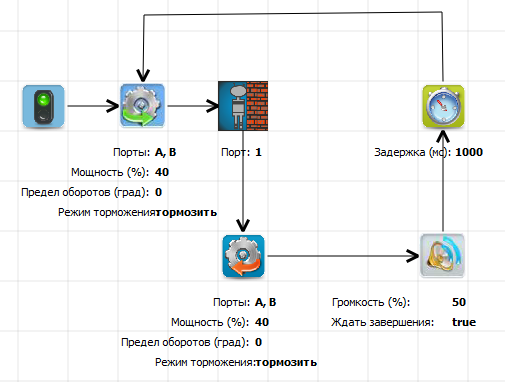
\includegraphics[width=0.6\textwidth]{programExample.png}
    \caption{Пример программы QReal:Robots}
    \label{programExample}
  \end{center}
\end{figure}

Приведём описание функциональности QReal:Robots, направленной на удовлетворение предложенных выше требований. Математические выражения в QReal:Robots могут задаваться в текстовой форме, в любом месте, где требуется численное значение, кроме того, есть отдельный блок <<функция>>, предназначенный для записи математического выражения. Имеется возможность использовать переменные и обращаться к текущим показаниям сенсоров прямо из выражения. В языке имеется поддержка алгоритмических конструкций --- ветвлений, циклов, параллельных потоков исполнения. Удобство пользовательского интерфейса QReal:Robots обеспечивается, во-первых, возможностями базовой технологии QReal, во-вторых, исследованиями удобства пользовательского интерфейса конкретно QReal:Robots. Базовая технология обеспечивает, например, распознавание жестов мышью, которое используется в QReal:Robots для быстрого рисования связей между блоками --- достаточно с зажатой правой кнопкой мыши провести линию между двумя блоками, чтобы соединить их. Проводилось анкетирование школьников по вопросам удобства использования QReal:Robots, выявленные замечания были исправлены.

Наличие развитых средств отладки является основным преимуществом QReal:Robots перед рассмотренными системами. Первое --- это возможность интерпретации программы на компьютере с дистанционным управлением роботом по Bluetooth или USB. При этом среда подсвечивает текущий исполняемый блок, визуализируя ход выполнения программы и давая возможность понять, какой блок вызвал ошибку. Второе --- наличие двухмерной модели робота, которая может быть использована как исполнитель программы вместо реального робота. Двухмерная модель имитирует трёхколёсную тележку, применяемую, например, в футболе роботов. Модель позволяет задавать расположение и тип сенсоров, и объекты реального мира, такие как стены и линии на полу, с которыми взаимодействуют сенсоры. Двухмерная модель позволяет отлаживать программы без использования настоящего робота, что делает цикл отладки гораздо быстрее и позволяет использовать QReal:Robots без доступа к роботу вообще, что может быть полезно для школ, пока не закупивших робототехнические конструкторы.

Среда QReal:Robots имеет генератор кода на языке C по диаграммам. Сгенерированный код можно скомпилировать и загрузить на робот для автономного исполнения, при этом его можно просматривать прямо в среде QReal. Среда изначально разрабатывалась для русскоязычной аудитории, поэтому не требует русификации, бесплатна (разрабатывается как продукт с открытым исходным кодом), продолжает активно развиваться силами сотрудников кафедры системного программирования СПбГУ.

\section*{Заключение}

Среда QReal:Robots была представлена на <<Открытых состязаниях Санкт-Петербурга по робототехнике>> 2012 года и на робототехническом фестивале <<Робофест 2012>> в Москве. В качестве доказательства применимости QReal:Robots к реальным задачам, решаемым школьниками, можно отметить, что команда студентов, принявшая  участие в соревнованиях с QReal:Robots, показала хорошие результаты. Им удалось занять места в середине таблицы несмотря на то, что многие участники использовали роботов, специально созданных для этой задачи. QReal:Robots представлялся также на стендовых докладах на этих соревнованиях, где вызвал большую заинтересованность у потенциальных пользователей. Было проведено анкетирование удобства пользовательского интерфейса, которое показало, что продукт достаточно хорош, чтобы вызывать у пользователей симпатию и желание им пользоваться.

Визуальное программирование роботов интересно с научной точки зрения тем, что является подходящей предметной областью для апробации средств поддержки предметно-ориентированного программирования. С одной стороны, использование визуальных языков программирования довольно широко распространено среди людей, занимающихся робототехникой, поэтому здесь можно рассчитывать на содержательное сравнение с существующими решениями и обратную связь от пользователей, уже знакомых с различными визуальными языками. С другой стороны, программирование роботов --- хороший пример предметной области, достаточно узкой, чтобы можно было получить заметное преимущество от создания для неё специализированного языка, и вместе с тем достаточно содержательной, чтобы такой специализированный язык был нетривиальным и мог бы послужить примером для исследования решений, применимых в других содержательных случаях. Описание предметной области, существующих разработок, тенденций и направлений развития средств визуального программирования роботов может быть важно как база для исследований в области предметно-ориентированного моделирования и для апробации технологий и методологий создания предметно-ориентированных визуальных языков. Детально описанный и практически полезный пример предметной области может быть полезен как ориентир и модельный пример при разработке DSM-платформы~\cite{dsmPlatforms}, и уже сейчас задача программирования роботов используется в таком качестве в проекте QReal~\cite{qReal}.

\begin{thebibliography}{9001}

  \bibitem{qReal} \emph{Терехов А.Н., Брыксин Т.А., Литвинов Ю.В., Смирнов К.К., Никандров Г.А., Иванов В.Ю., Такун Е.И.} Архитектура среды визуального моделирования QReal // Системное программирование. Вып. 4. СПб.: Изд-во СПбГУ. 2009, С. 171--196.

  \bibitem{mythicalManMonth} \emph{Брукс Ф.} Мифический человеко-месяц, или Как создаются программные системы, Символ-Плюс, 2010. 304 С.

  \bibitem{dsmPlatforms} \emph{Павлинов А.А., Кознов Д.В., Перегудов А.Ф., Бугайченко Д.Ю., Казакова А.С., Чернятчик Р.И., Иванов А.Н..} О средствах разработки проблемно-ориентированных визуальных языков // Системное программирование. 2006. Т. 2. № 1. С. 116--141.

  \bibitem{robik} \emph{Звенигородский Г.А.} Описание языка Робик, URL: http://ershov.iis.nsk.su/archive/eaindex.asp?lang=1\&did=7639 

  \bibitem{filippov} \emph{Филиппов С.А.} Робототехника для детей и родителей, Наука, 2011. 264 с.

  \bibitem{robots} \emph{Брыксин Т.А., Литвинов Ю.В.} Среда визуального программирования роботов QReal:Robots // Материалы международной конференции <<Информационные технологии в образовании и науке>>. Самара. 2011. С. 332--334.

  \bibitem{logo} MyRobot, Язык программирования Лого, URL: http://myrobot.ru/logo/aboutlogo.php   

  \bibitem{logoTurtle} cyberneticzoo.com, 1969 – The Logo Turtle – Seymour Papert et al, URL: http://cyberneticzoo.com/?p=1711 

  \bibitem{mrdsAtMySpace} \emph{Michael S. Scherotter}, CCR at MySpace, URL: http://channel9.msdn.com/Shows/Communicating/CCR-at-MySpace 

  \bibitem{legoNxt} Lego Mindstorms homepage, URL: http://mindstorms.lego.com/en-us/Default.aspx

  \bibitem{mrds} Microsoft Robotics Developer Studio homepage, URL: http://www.microsoft.com/robotics/ 

  \bibitem{robolab} \emph{Portsmore, Merredith} ROBOLAB: Intuitive Robotic Programming Software to Support Life Long Learning, APPLE Learning Technology Review, Spring/Summer 1999.

  \bibitem{rtst} \emph{Терехов А.Н.}  RTST-технология программирования встроенных систем реального времени. // Записки семинара Кафедры системного программирования "Case-средства RTST++". 1998. С. 3.

  \bibitem{real} \emph{Terekhov A.N., Romanovskii K.Yu., Koznov D.V., Dolgov P.S., Ivanov A.N.} RTST++: Methodology and a CASE Tool for the Development of Information Systems and Software for Real-time Systems. Programming and Computer Software. 1999. Vol. 25. № 5. P. 276--281. 

  \bibitem{comapping} \emph{Koznov D., Pliskin M.} COMPUTER-SUPPORTED COLLABORATIVE LEARNING WITH MIND-MAPS. Communications in Computer and Information Science. 2008. Vol. 17 CCIS. P. 478--489.

  \bibitem{viDip} \emph{Кознов Д.В., Перегудов А.Ф., Бугайченко Д.Ю., Чернятчик Р.И., Казакова А.С., Павлинов А.А.} Визуальная среда проектирования систем телевизионного вещания // Системное программирование. 2006. Т. 2. № 1. С. 142--168.

  \bibitem{nxtG} LEGO web site, NXT-G download page, URL: http://service.lego.com/en-us/helptopics/?questionid=2655
	
\end{thebibliography}

\end{document}
